\documentclass[a4paper,11pt]{article}
\usepackage{lecturenotes}
\usepackage{multicol}
\usepackage{changepage}
\usepackage{xcolor}
\usepackage{makecell}
\lectureheader{ELE727}{1}



\begin{document}

\notesection{NMOS/CMOS Device Structure}
\begin{figure}[htbp]
    \centering
    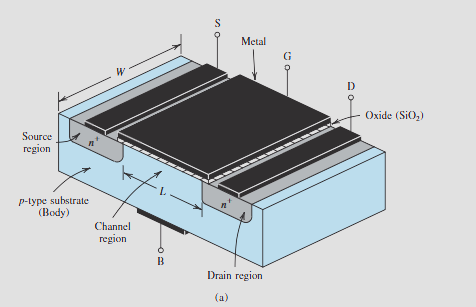
\includegraphics[width=0.5\linewidth]{figures/nmos-device-structure.png}
    \caption{NMOS Device Structure}
    \label{fig:NMOS-Device-Structure}
\end{figure}

\begin{figure}[htbp]
    \centering
    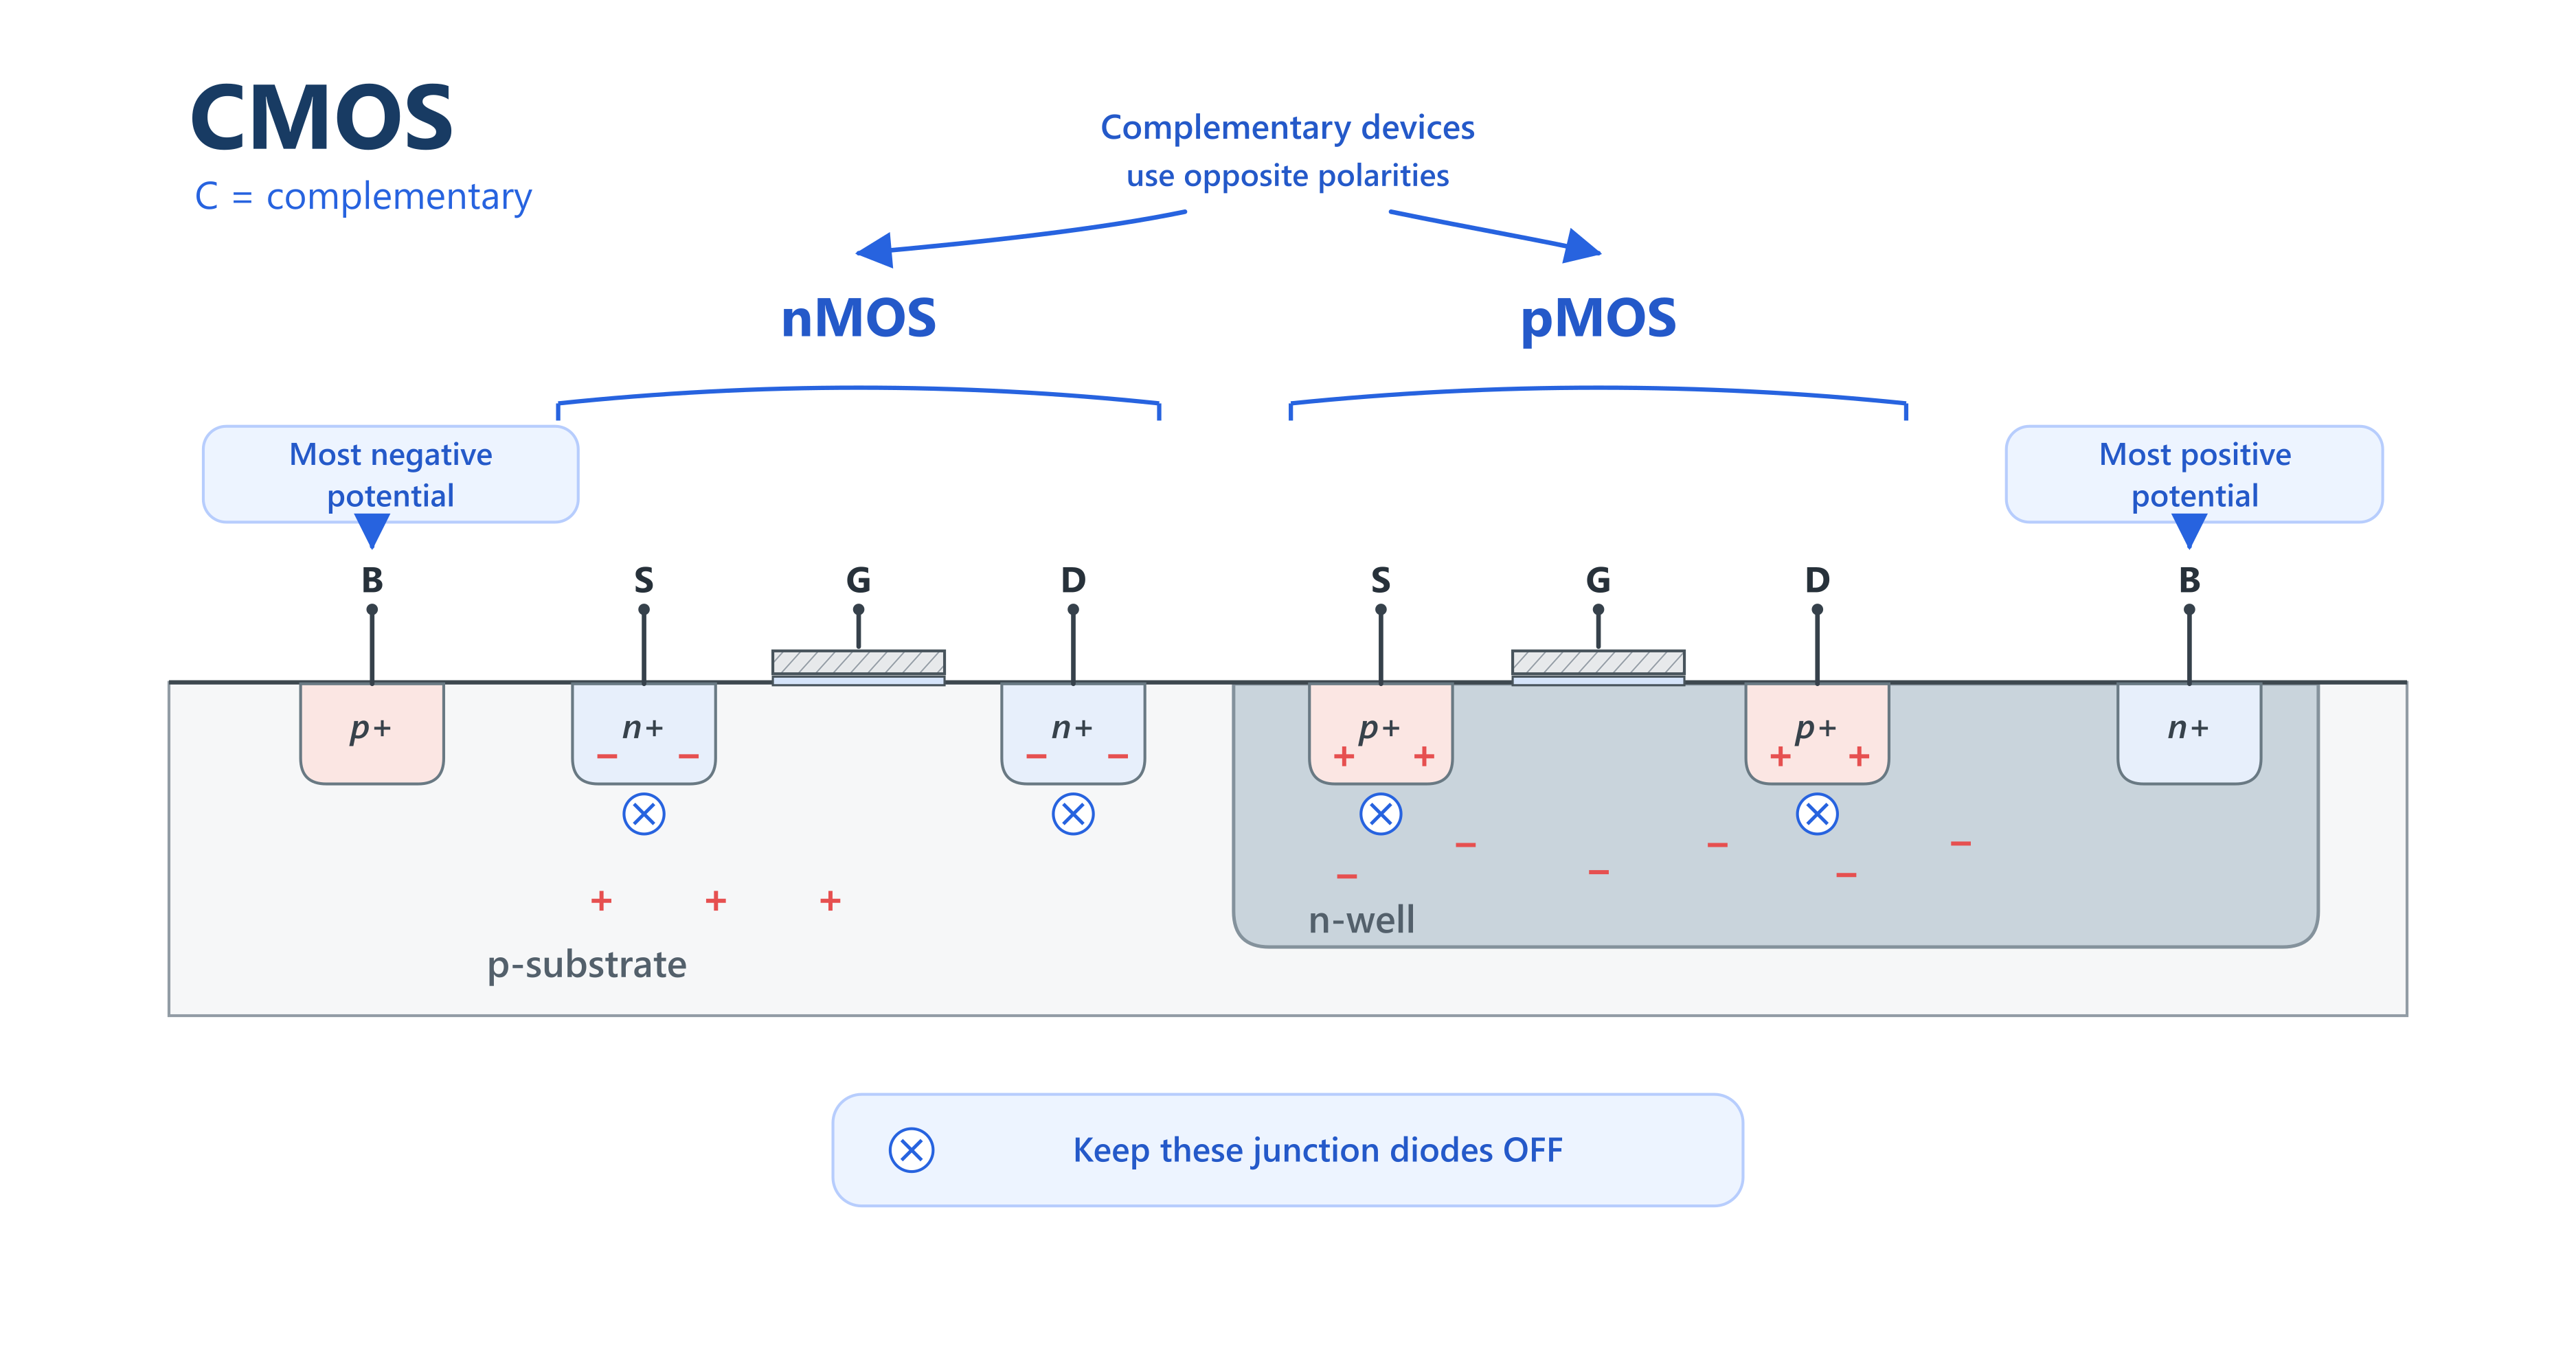
\includegraphics[width=0.8\linewidth]{figures/cmos-device-annotated.png}
    \caption{CMOS Device Structure}
    \label{fig:CMOS-Device-Structure}
\end{figure}


To differentiate between a PMOS and NMOS transistor, simply look at the arrow at the source point of the transistor device
\begin{multicols}{2}


    \begin{notecircuit}[scale=1.2,transform shape]{NMOS Symbol}
        \draw (0,0) node[nmos,bulk,arrowmos] (mos) {};

        \node[left]  at (mos.G) {$G$};
        \node[above] at (mos.D) {$D$};
        \node[below] at (mos.S) {$S$};
        \node[right] at (mos.bulk) {$B$};

        % V_GS: + at G, - at S
        \coordinate (vgsPlus)  at ([xshift=-8mm]mos.G);
        \coordinate (vgsMinus) at (vgsPlus |- mos.S);

        \node[red] at (vgsPlus)  {$+$};
        \node[red] at (vgsMinus) {$-$};
        \node[red,anchor=east,xshift=-2mm]
        at ($(vgsPlus)!0.5!(vgsMinus)$) {$V_{GS}$};

        % V_DS: + at D, - at S
        \coordinate (vdsPlus)  at ([xshift=10mm]mos.D);
        \coordinate (vdsMinus) at (vdsPlus |- mos.S);

        \node[green!50!black] at (vdsPlus)  {$+$};
        \node[green!50!black] at (vdsMinus) {$-$};
        \node[green!50!black,anchor=west,xshift=2mm]
        at ($(vdsPlus)!0.5!(vdsMinus)$) {$V_{DS}$};
    \end{notecircuit}

    \vspace{0.5cm}

    \begin{notecircuit}[scale=1.2,transform shape]{PMOS Symbol}
        \draw (0,0) node[pmos,bulk,arrowmos] (mos) {};

        \node[left]  at (mos.G) {$G$};
        \node[above] at (mos.S) {$S$};
        \node[below] at (mos.D) {$D$};
        \node[right] at (mos.bulk) {$B$};

        % V_SG: + at S, - at G
        \coordinate (vsgMinus) at ([xshift=-8mm]mos.G);
        \coordinate (vsgPlus)  at (vsgMinus |- mos.S);

        \node[red] at (vsgPlus)  {$+$};
        \node[red] at (vsgMinus) {$-$};
        \node[red,anchor=east,xshift=-2mm]
        at ($(vsgPlus)!0.5!(vsgMinus)$) {$V_{SG}$};

        % V_SD: + at S, - at D
        \coordinate (vsdPlus)  at ([xshift=10mm]mos.S);
        \coordinate (vsdMinus) at (vsdPlus |- mos.D);

        \node[green!50!black] at (vsdPlus)  {$+$};
        \node[green!50!black] at (vsdMinus) {$-$};
        \node[green!50!black,anchor=west,xshift=2mm]
        at ($(vsdPlus)!0.5!(vsdMinus)$) {$V_{SD}$};
    \end{notecircuit}
\end{multicols}

\notesection{Regions of Operation}

\begin{notetable}{X X}{\textbf{Region} & \textbf{Condition}}
    OFF* & $V_{GS} < V_{TH}$ \\
    TRIODE & $V_{GS} \geq V_{TH}$ AND\newline
    $V_{DS} < V_{DS,SAT} = (V_{GS}-V_{TH})^*$ AND\newline
    $V_{DS} << V_{DS,SAT}$ (DEEP TRIODE) \\
    SATURATION & $V_{GS} \geq V_{TH}$ AND\newline
    $V_DS \geq V_{DS,Sat}$ \\
\end{notetable}
\begin{adjustwidth}{1.5em}{1.5em}
    \small
    *For $V_{GS} > 0V \rightarrow I_D \neq 0 \rightarrow$ Subthreshhold conduction \\
    **$V_{DS,Sat}$ also known as \textbf{overdrive voltage}, $V_OV$ or $V_OD$ and the \textbf{effective voltage}, $V_{EFF}$ \\ \\
\end{adjustwidth}

In Analog Circuit design, we want the transistors to be in the saturation region 95\% of the time. For that to occur, the following has to be satifised:
\notedefinition{Saturation Region}{$V_{GS} \geq V_{TH}$ and $V_{DS} >> (V_{GS} - V_{TH})$}


\notesection{Triode Region}

\begin{figure}[htbp]
    \centering
    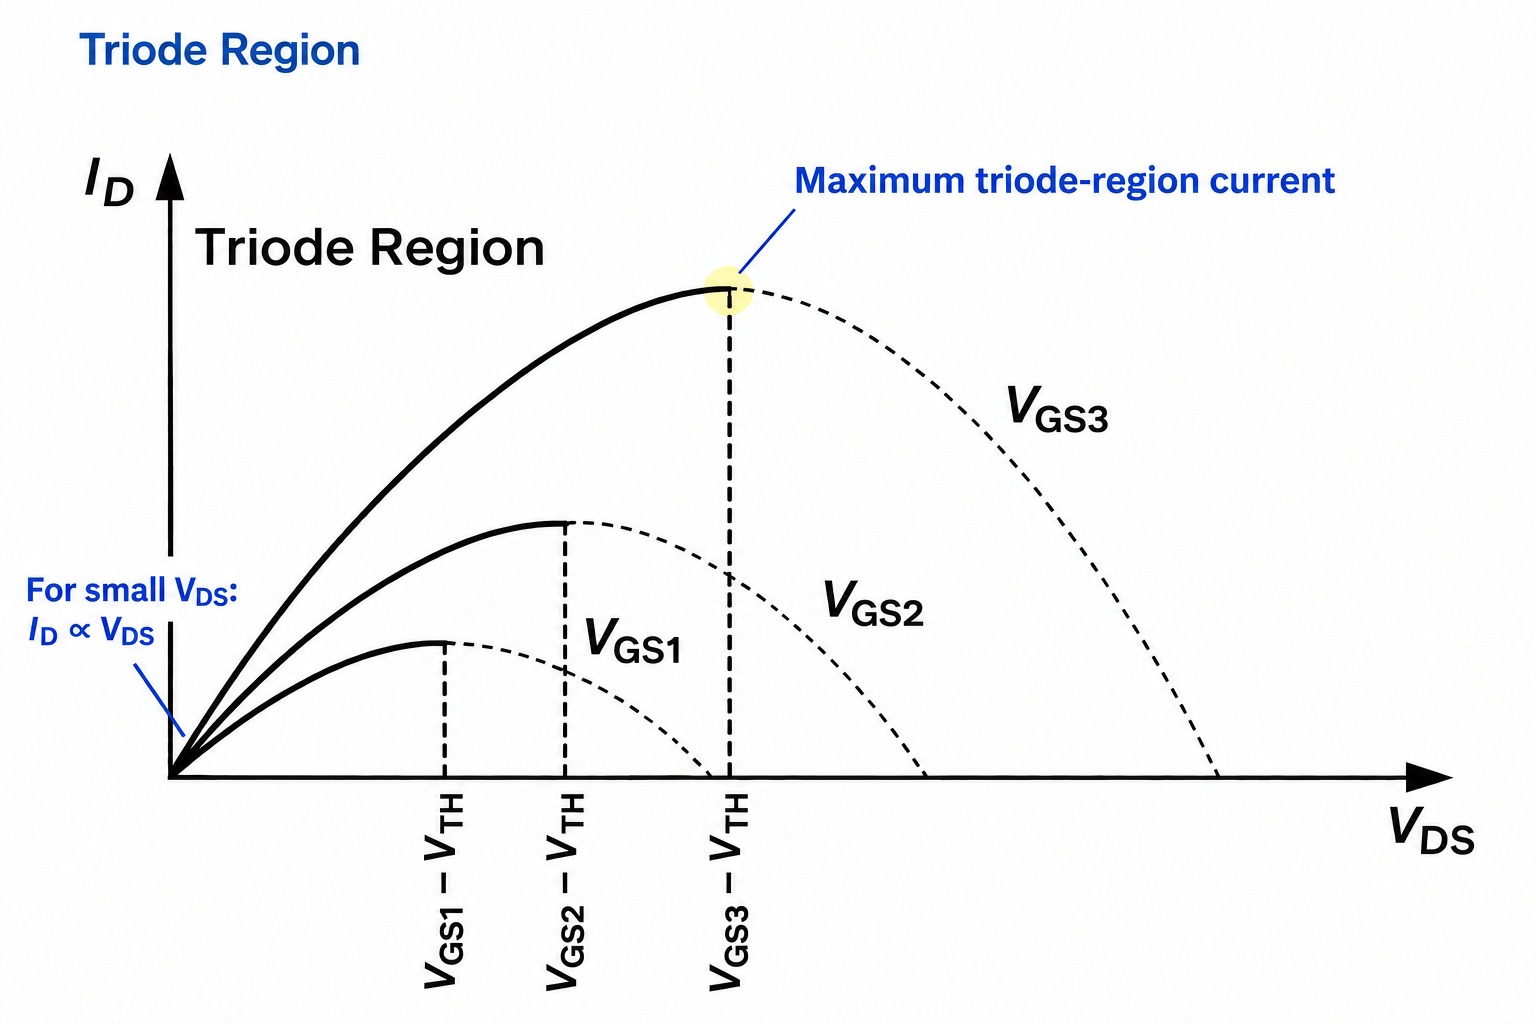
\includegraphics[width=0.8\linewidth]{figures/mosfet-triode-region-annotated.png}
    \caption{Triode Region}
    \label{fig:Triode-region}
\end{figure}

In the ideal case: $\frac{\partial I_D}{\partial V_{DS}} = 0$ when $V_{DS} = V_{GS} - V_{TH}$

\keyequation{$I_{D}$ in Triode Region}{I_D = \mu_n C_{OX} \frac{W}{L}[(V_{GS}-V_{TH}) V_{DS} - \frac{1}{2}V_{DS}^2)]}[
    \begin{description}
        \item[$\mu_n$] - Electron Mobility in N-type
        \item[$C_{OX}$] - Gate-Oxide Capacitance
    \end{description}
]

\notesection{Deep Triode Region}

\begin{figure}[htbp]
    \centering
    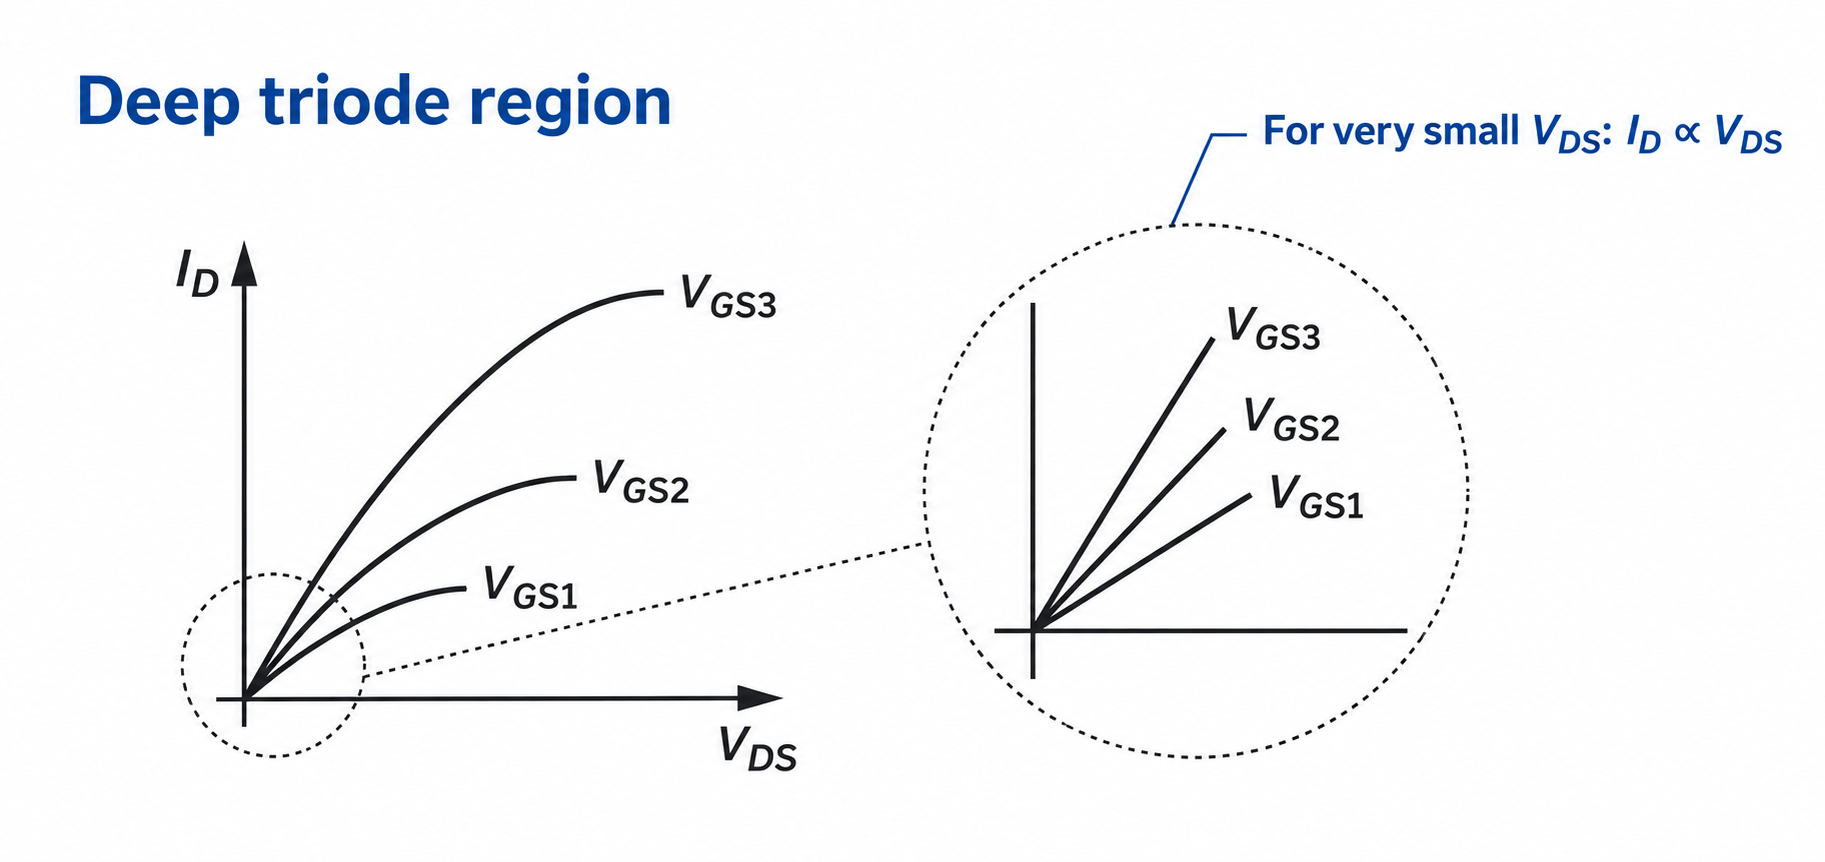
\includegraphics[width=0.8\linewidth]{figures/mosfet-deep-triode-region.png}
    \caption{Triode Region}
    \label{fig:Deep-Triode-region}
\end{figure}
\keyequation{$I_D$ in Deep Triode}{I_D = \mu_n C_{ox} \frac{W}{L} (V_{GS} - V_{TH}) V_{DS}}
\vspace{0.5cm}
\notedefinition{Behaviour of a MOSFET in Deep-Triode}{A MOSFET in the deep triode region acts as a voltage-controlled resistor}

Keep in mind that $R = \frac{V}{I}$ we are then able to determine the \textit{on resistance} of the MOSFET by re-arranging the equation.

\begin{notederivation}{On Resistance of a MOSFET in Deep-Triode}
    & I_D = \mu_n C_{ox} \frac{W}{L} (V_{GS} - V_{TH}) V_{DS} && \qquad \text{Drain Current} \\
    & \frac{V_{DS}}{I_D} = \frac{1}{\mu_n C_{ox} \frac{W}{L} (V_{GS} - V_{TH}) V_{DS}} && \qquad \text{Definition of On Resistance} \\
\end{notederivation}

\keyequation{$R_ON$ in Deep Triode}{R_{ON} = \frac{1}{\mu_n C_{ox} \frac{W}{L} (V_{GS} - V_{TH}) V_{DS}}}

\notesection{Saturation Region}

\begin{figure}[htbp]
    \centering
    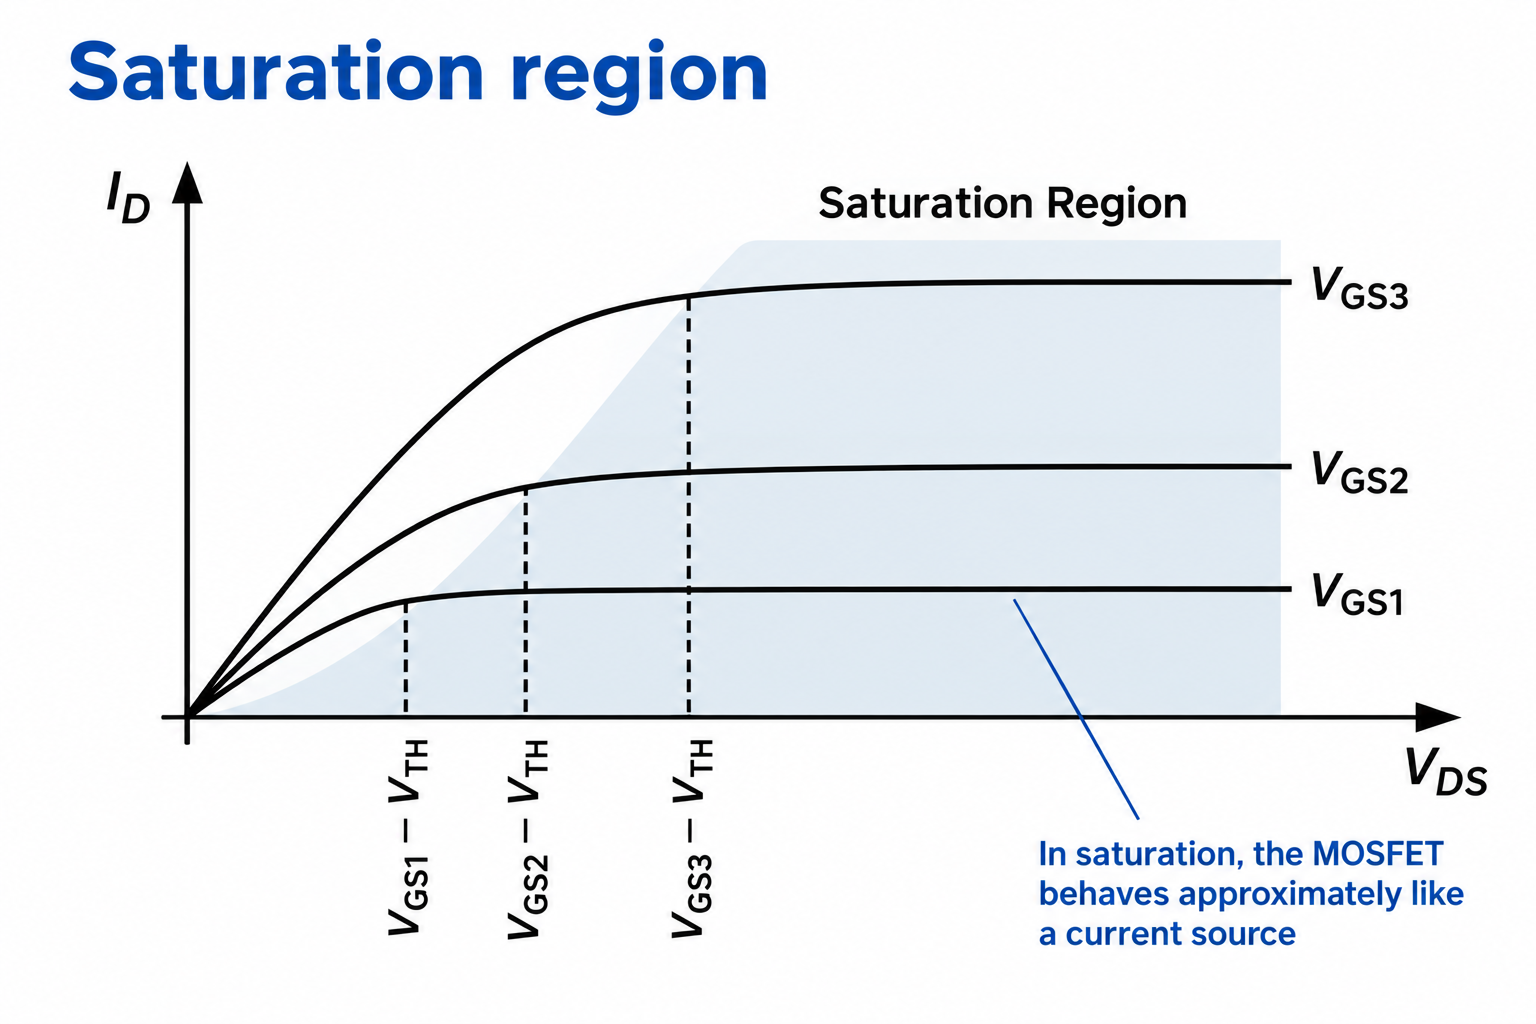
\includegraphics[width=0.8\linewidth]{figures/mosfet-saturation-region.png}
    \caption{Satration Region}
    \label{fig:Saturation-Region}
\end{figure}

When $V_{DS} \geq V_{GS} - V_{TH}$, $I_D$ is indepdent of $V_{DS}$ in the ideal case ($I_D$ saturates to a \textit{"constant"} value)

The equation for drain current is then:
\keyequation{$I_D$ in Saturation}{I_D = \frac{1}{2} \mu_n C_{OX} \frac{W}{L} (V_{GS} - V_{TH})^2}[
    This is also known as the \textcolor{red}{\textbf{square law}}
]
\notedefinition{Behaviour of MOSFET in Saturation}{Behaves as a voltage controlled current source (controlled by $V_{GS}$)}
\begin{notetable}{X c c c}{\textbf{PARAMETER} & \textbf{Unit} & \textbf{nCH} & \textbf{nPH}}
    $\mu_0 C_{OX}$\newline \textit{Physical Transconductance} & $\frac{\mu A}{V^2}$ & 250 & 70 \\
    $2 \phi_f$\newline \textit{Fermi Level}, also related to transconductance and voltage threshhold & V & 0.8 & 0.8 \\
\end{notetable}

\begin{figure}[htbp]
    \centering
    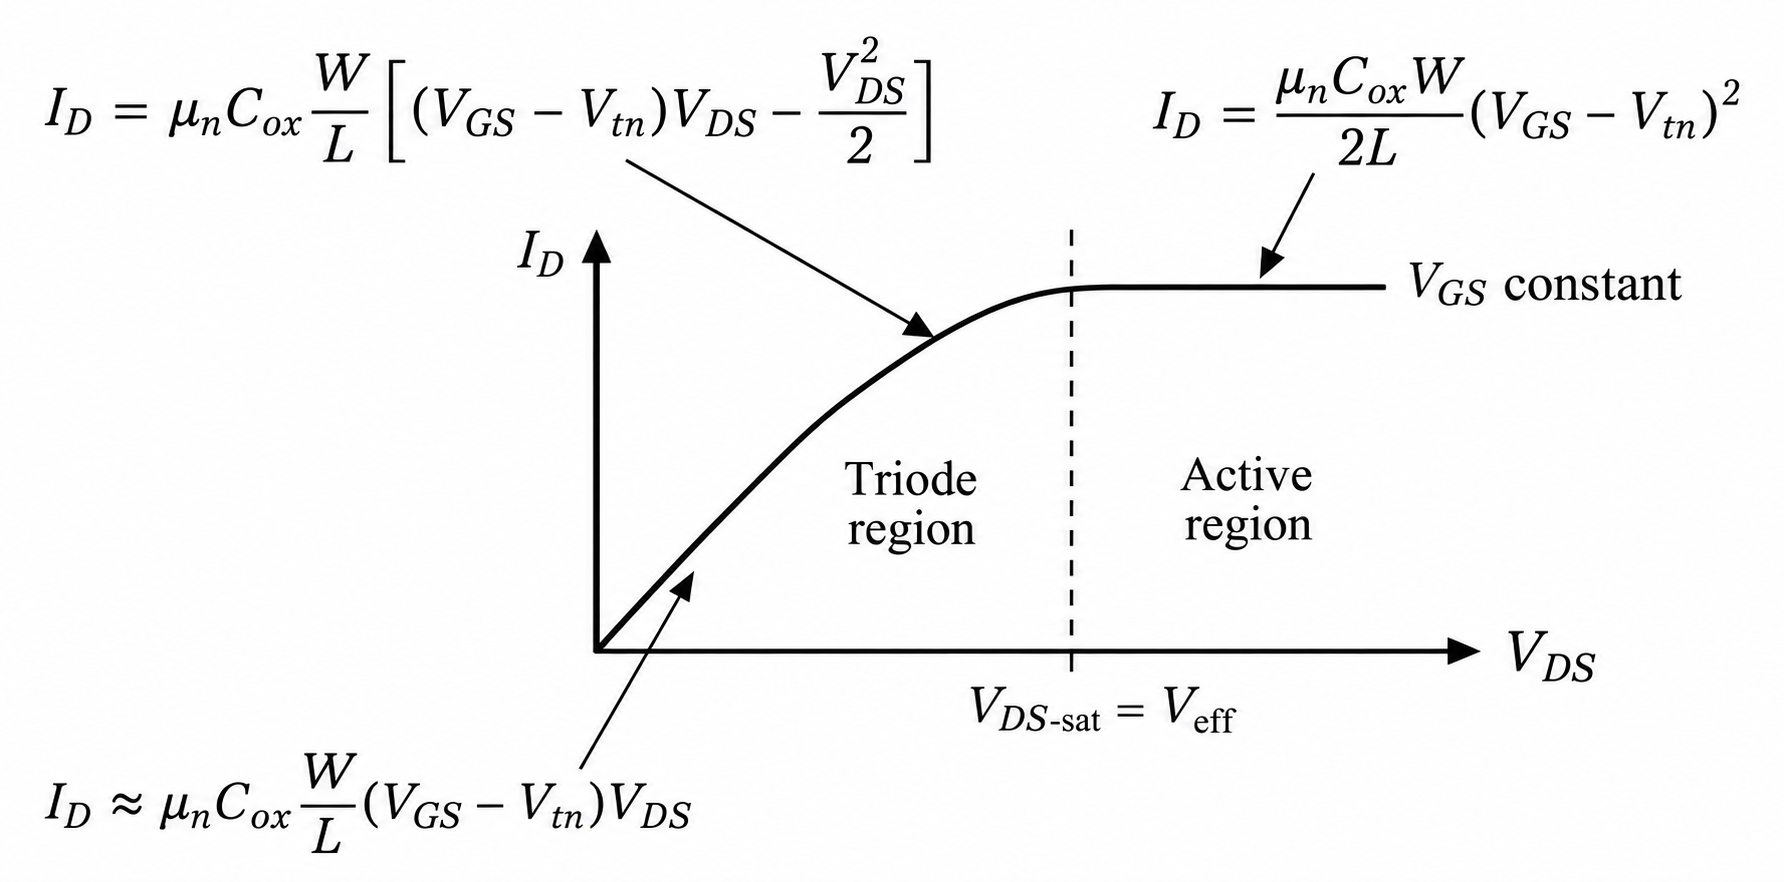
\includegraphics[width=0.8\linewidth]{figures/mosfet-operating-regions-equations.png}
    \caption{Strong Inversion}
    \label{fig:Strong-Inversion}
\end{figure}
\notesection{MOS Transconductance, $g_m$}

\notedefinition{Transconductance}{Conductance across the device in saturation}

Remember that: $I_d = \frac{1}{2} \mu_x C_{OX} \frac{W}{L} (V_{GS} - V_{TH})^2$, and that by defintion: $g_n = \frac{\partial I_D}{\partial V_{GS}}$. By using this as the
base defintion of transconductance, we can emphasize three different representations of transconductance.
\begin{notetable}{l X c}{\textbf{In terms of} & \textbf{Equation} & \textbf{Notes}}
    \rule{0pt}{2.8ex}Standard & $g_n = \mu_n C_{ox} \frac{W}{L} (V_{GS} - V_{TH}) [S \quad \text{or} \quad \frac{A}{V}]$ & N/A \\
    \rule{0pt}{2.8ex}In terms of $I_D$ and $\frac{W}{L}$ & $g_n = \sqrt{2 \mu_n C_ox \frac{W}{L} I_D}$ & quadratic w.r.t current \\
    \rule{0pt}{2.8ex}In terms of $V_{OV}$ and $I_D$ & $g_n = \frac{2 I_D}{(V_{GS} - V_{TH})} = \frac{2 I_D}{V_{OV}}$ & \makecell[c]{design eqn.\\(strong inversion only)} \\
\end{notetable}

\begin{itemize}
    \item Typically $g_n$ is derived from specifications such as desired gain
    \item Only valid during strong inversion (deep in saturation)
\end{itemize}

\notesection{MOS Output Resistance, $r_o$ and Channel Length Modulation Coeffecient, $\lambda$}
\begin{figure}[htbp]
    \centering
    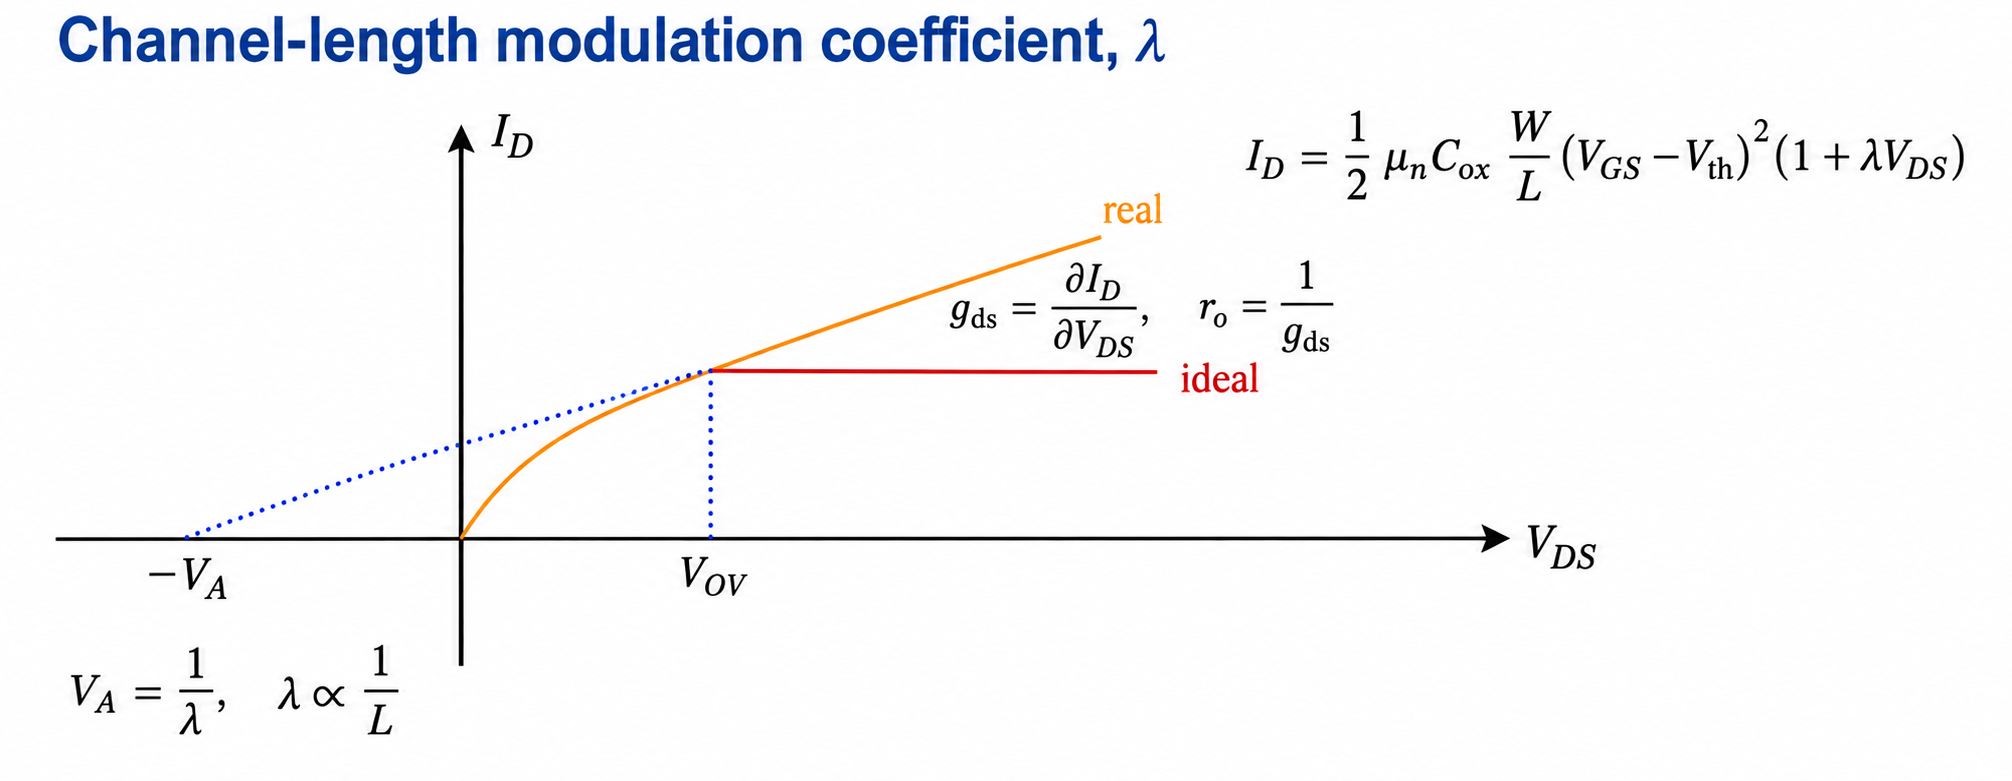
\includegraphics[width=0.8\linewidth]{figures/mosfet-channel-length-modulation.png}
    \caption{Non-ideal $I_D$ vs. $V_{DS}$ Graph}
    \label{fig:Non-ideal-I-and-V}
\end{figure}

\notedefinition{CLM Proportionality}{$\lambda = \frac{1}{V_A} \propto \frac{1}{L}$}

\keyequation{Output Resistance $r_o$}{
    \begin{aligned}
        r_o & = (\frac{\partial I_D}{\partial V_{DS}})^-1                               \\
            & = \frac{1}{\frac{1}{2}\mu_n C_{OX} \frac{W}{L} (V_{GS}-V_{TH})^2} \lambda \\
            & \thickapprox \frac{1}{\lambda I_D}
    \end{aligned}
}

\notesection{Body Effect - $V_SB > 0$}

\keyequation{Threshhold Voltage as a Result of Body Effect}{V_{TH} = V_{TH0} + \gamma (\sqrt{2 \phi_F + V_{SB}} - \sqrt{|2\phi_F|})}[
    Note that: $\gamma = \frac{\sqrt{2q \epsilon_{si} N_{sub}}}{C_{OX}}$\newline
    \vspace{0.5cm}
    and that the threshhold voltage is related to the voltage difference between source and body
]

\par\medskip
\noindent
\begin{minipage}[t]{0.31\linewidth}
    \centering
    \textbf{Case 1}\par\smallskip
    {\small $V_{SB} = 0 \rightarrow V_{TH} = V_{TH0}$}\par\medskip
    \begin{circuitikz}[scale=0.9, transform shape]
        \draw (0,0) node[nmos,bulk,arrowmos] (mos) {};
    \end{circuitikz}
\end{minipage}\hfill
\begin{minipage}[t]{0.31\linewidth}
    \centering
    \textbf{Case 2}\par\smallskip
    {\small $V_{SB} > 0 \rightarrow V_{TH} > V_{TH0}$}\par\medskip
    \begin{circuitikz}[scale=0.9, transform shape]
        \draw (0,0) node[nmos, bulk, arrowmos] (M1) {};

        \draw (M1.G) -- ++(-0.7,0)
        node[ocirc] {};

        \draw[->] (M1.D) -- ++(0,0.75);

        % invert places + at the source and - at ground
        \draw (M1.S)
        to[american voltage source, invert, l_={$V_S$}]
        ++(0,-1.3)
        node[ground] {};

        \draw (M1.bulk) -- ++(0.6,0)
        -- ++(0,-0.75)
        node[ground] {};
    \end{circuitikz}
\end{minipage}\hfill
\begin{minipage}[t]{0.31\linewidth}
    \centering
    \textbf{Case 3}\par\smallskip
    {\small $V_{SB} < 0 \rightarrow V_{TH} < V_{TH0}$}\par\medskip
    \begin{circuitikz}[scale=0.9, transform shape]
        \draw (0,0) node[nmos, bulk, arrowmos] (M1) {};

        % Gate
        \draw (M1.G) -- ++(-0.7,0)
        node[ocirc] {};

        % Drain
        \draw[->] (M1.D) -- ++(0,0.75);

        % Source grounded
        \draw (M1.S) -- ++(0,-0.4)
        node[ground] {};

        % Body-bias supply: V_BS = V_B - V_S
        \draw (M1.bulk) -- ++(0.65,0)
        to[american voltage source, invert, l_={$V_{BS}$}]
        ++(0,-1.3)
        node[ground] {};
    \end{circuitikz}
\end{minipage}
\par\medskip

\notesection{Body Transconductance, $g_mb$}

\begin{notederivation}{Body Transconductance}
    & I_D = \frac{1}{2}C_{OX}\frac{W}{L}(V_{GS} V_{TH})^2 && \qquad \text{Drain Current} \\
    & g_{mb} = \frac{\partial I_D}{\partial V_{BS}} = \frac{\partial I_D}{\partial V_{TH}}(- \frac{\partial I_D}{\partial V_{SB}}) && \qquad \text{Definition of Transconductance} \\
\end{notederivation}

\keyequation{Body Transconductance, $g_{mb}$}{
g_{mb} = -\mu_n C_{OX} \frac{W}{L} (V_{GS} - V_{TH}) \cdot [ - \frac{\gamma}{2} (2 \phi_F + V_{SB}^{-\frac{1}{2}}] \enspace = \enspace \eta g_m
}
\notesection{MOSFET Small-signal Equivalent [in saturation][low-frequency model]}
\begin{center}
    \begin{circuitikz}[american, scale=1.1, transform shape]
        % Drain and source rails
        \draw (0,2) -- (7.5,2)
        node[ocirc] {}
        node[right] {$D$};

        \draw (-2,0) -- (7.5,0)
        node[ocirc] {}
        node[right] {$S$};

        % Gate terminal and V_GS polarity
        \draw (-3.2,2)
        node[ocirc] {}
        node[left] {$G$}
        -- (-2,2);

        \node at (-2,1.75) {$+$};
        \node at (-2,1) {$V_{GS}$};
        \node at (-2,0.25) {$-$};

        % g_m V_GS current source
        \draw (0,2) node[circ] {}
        to[I] (0,0) node[circ] {};

        \node[anchor=west] at (0.55,1)
        {$g_mV_{GS}$};

        % Output resistance
        \draw (3,2) node[circ] {}
        to[R] (3,0) node[circ] {};

        \node[anchor=west] at (3.5,1)
        {$r_o$};

        % Body-effect current source
        \draw (6,2) node[circ] {}
        to[I] (6,0) node[circ] {};

        \node[anchor=west] at (6.55,1)
        {$g_{mb}V_{BS}$};

        % Body terminal and V_BS polarity
        \draw (-3.2,-1.55)
        node[ocirc] {}
        node[left] {$V_B$}
        -- (-2,-1.55);

        \node at (-2,-0.25) {$-$};
        \node at (-2,-0.8) {$V_{BS}$};
        \node at (-2,-1.3) {$+$};
    \end{circuitikz}
\end{center}

If $\lambda = 0 \rightarrow$ No chanel-lenth modulation $\rightarrow r_0 \approx \infty$ then $\gamma = 0 \rightarrow g_{mb} V_{SB} = 0$

\begin{center}
    \begin{circuitikz}[american, scale=1.15, transform shape]
        % Body input
        \draw (-3.2,1.8)
        node[ocirc] {}
        node[left] {$B$}
        -- (-1.6,1.8);

        % V_BS polarity
        \node at (-1.6,1.5) {$+$};
        \node at (-1.6,0.9) {$V_{BS}$};
        \node at (-1.6,0.3) {$-$};

        % Common source connection
        \draw (-3.2,0) -- (0,0);

        % Body-effect controlled current
        \draw (0,1.8)
        to[I] (0,0);

        \node[anchor=west] at (0.55,0.9)
        {$g_{mb}V_{BS}$};

        % Drain output
        \draw (0,1.8) -- (2.6,1.8)
        node[ocirc] {}
        node[right] {$D$};

        % Source output
        \draw (0,0) -- (2.6,0)
        node[ocirc] {}
        node[right] {$S$};
    \end{circuitikz}
\end{center}

\end{document}
